\documentclass[12pt,a4paper]{article}

% =========================================================
% PACKAGES
% =========================================================
\usepackage[margin=1in]{geometry}
\usepackage{setspace}
\usepackage{graphicx}
\usepackage{float}
\usepackage{booktabs}
\usepackage{longtable}
\usepackage{array}
\usepackage{tabularx}
\usepackage{multirow}
\usepackage{enumitem}
\usepackage{xcolor}
\usepackage{pdflscape}
\usepackage{microtype}
\usepackage{ragged2e}
\usepackage{titlesec}
\usepackage{etoolbox}
\usepackage{tikz}
\usepackage{amsmath}
\usepackage{amssymb}
\usepackage{hyperref}
\usepackage{csquotes}

% APA 7 bibliography
\usepackage[
    style=apa,
    backend=biber,
    sorting=nyt
]{biblatex}

\addbibresource{references.bib}

% TikZ libraries
\usetikzlibrary{
    arrows.meta,
    positioning,
    shapes.geometric,
    fit,
    backgrounds
}

% =========================================================
% DOCUMENT SETTINGS
% =========================================================
\onehalfspacing

\hypersetup{
    colorlinks=true,
    linkcolor=black,
    citecolor=black,
    urlcolor=black
}

\setlength{\parindent}{0pt}
\setlength{\parskip}{6pt}
\newcolumntype{P}[1]{>{\raggedright\arraybackslash}p{#1}}

\titleformat{\section}{\Large\bfseries\color{black}}{\thesection.}{0.5em}{}
\titleformat{\subsection}{\large\bfseries}{\thesubsection}{0.5em}{}
\pretocmd{\section}{\clearpage}{}{}

\pagestyle{plain}

% =========================================================
% TITLE
% =========================================================

\begin{document}
\pagenumbering{gobble}

\begin{titlepage}
\centering

\vspace*{1.1cm}

{\large\color{black!65}\textsc{Fall Semester 2026--27}\par}
\vspace{0.35cm}
{\Large\bfseries\color{black}BITE308L: ARTIFICIAL INTELLIGENCE\par}

\vspace{1.1cm}
{\color{black}\rule{0.88\textwidth}{1.2pt}\par}
\vspace{0.7cm}

\colorbox{black}{%
    \parbox{0.30\textwidth}{%
        \centering\color{white}\large\bfseries REVIEW--1
    }%
}

\vspace{1cm}

{\fontsize{25}{31}\selectfont\bfseries\color{black!85}
Adaptive Security Awareness\\[0.18cm]
Training System\par}

\vspace{0.55cm}

{\Large\color{black}
Using Reinforcement Learning and\\[0.12cm]
LLM-Based Scenario Generation\par}

\vspace{0.7cm}
{\color{black}\rule{0.88\textwidth}{1.2pt}\par}

\vspace{1.3cm}

{\large\bfseries Submitted by\par}
\vspace{0.55cm}

\renewcommand{\arraystretch}{1.45}
\begin{tabular}{@{}>{\bfseries}r l@{}}
Student Name & Register Number \\
\midrule
Dhruv Jain & 24BIT0379 \\
Akshat Pandey & 24BIT0395
\end{tabular}

\end{titlepage}

\pagenumbering{roman}
\tableofcontents
\clearpage
\pagenumbering{arabic}


% =========================================================
% 1. ABSTRACT
% =========================================================

\section{Abstract}

Phishing remains difficult to prevent because it targets human
judgement as much as technical weaknesses. Most security-awareness
programs rely on a fixed collection of examples and present broadly
similar material to every employee. In practice, however, one person
may react strongly to urgency while another may be more influenced by
authority, invoices, or requests for credentials.

This project proposes an Adaptive Security Awareness Training System
that brings together reinforcement learning, large language model
(LLM) scenario generation, and lightweight behavior classification in
a closed feedback loop. The system treats urgency, authority
impersonation, fake invoices, and credential requests as arms in a
multi-armed bandit. During each training round, the bandit chooses a
tactic using the evidence gathered from earlier interactions.

The chosen tactic, together with the employee's role and context, is
then passed to an LLM to create a new simulated phishing scenario. The
employee or simulator responds by clicking, ignoring, or reporting the
message. A behavior classifier interprets this response, and the reward
module converts it into feedback for the bandit. As more interactions
are recorded, the system gradually changes which tactics it presents
and gives greater attention to the areas that require more training.

The project is limited to a controlled, consent-based simulation; it
does not send real phishing emails or collect real credentials. Its
performance will be assessed by comparing the adaptive policy with a
random tactic-selection baseline. The expected result is a practical
prototype that generates varied scenarios, personalizes training, and
makes the adaptation process measurable.


% =========================================================
% 2. PROBLEM STATEMENT
% =========================================================

\section{Problem Statement}

Many security-awareness programs follow a fixed sequence of
pre-written phishing examples. Although this approach is easy to
deploy, it does not learn from the way an individual employee responds.

Susceptibility is rarely uniform. An employee who easily recognizes a
fake invoice may still respond to a message that creates urgency or
appears to come from a senior manager. A fixed training plan can
therefore spend time repeating familiar lessons while giving too little
attention to the employee's weaker areas.

Therefore, the problem addressed by this project is:

\begin{quote}
\textit{How can an artificial-intelligence-based security awareness
training system dynamically identify an employee's comparatively weak
social-engineering tactic and adapt subsequent training scenarios using
reinforcement learning and LLM-based scenario generation?}
\end{quote}

To address this problem, the project links a multi-armed-bandit agent,
an LLM scenario generator, a simulated employee model, and a reward
mechanism. Together, these components form a loop in which every
response influences the scenario selected for a later round.


% =========================================================
% 3. MOTIVATION
% =========================================================

\section{Motivation}

The project is motivated by a simple limitation of conventional
awareness training: the same lesson does not have the same value for
every employee. Phishing decisions are shaped by context, including
urgency, authority, financial pressure, and requests for sensitive
information. Training is likely to be more useful when it responds to
these differences instead of treating every learner in the same way.

Reinforcement learning is well suited to this setting because training
takes place over a sequence of decisions. The system chooses a tactic,
observes the response, and uses that feedback when choosing the next
scenario. Here, the action is the selected social-engineering tactic,
the observation is the employee's simulated behavior, and the reward
captures the value of that interaction for the training policy.

LLMs complement this decision process by producing fresh scenarios for
the selected tactic and employee context. This reduces dependence on a
small set of repeated templates. Combining adaptive selection with
dynamic generation creates a training experience that can evolve from
one round to the next.


% =========================================================
% 4. LITERATURE SURVEY AND GAP IDENTIFICATION & OBJECTIVES
% =========================================================

\section{Literature Survey}

Existing phishing research can be grouped into several related areas:
technical detection, human susceptibility, awareness training, and
adaptive decision-making. Reinforcement learning has mainly been used
to detect phishing websites or network intrusions, where an agent
learns from repeated feedback \parencite{ariyadasa2024,chatterjee2019,kheddar2024}.
Related work has used neural networks and hybrid machine-learning
methods to identify phishing emails, malicious URLs, and other harmful
online content \parencite{smadi2018,jabbar2025,patil2025}.

The growth of large language models has introduced a different
challenge. LLMs can produce convincing, context-aware phishing content
and can personalize messages at scale \parencite{bethany2026,czybik2026}.
While this capability increases the threat, it can also be used
defensively to create varied and realistic awareness exercises in a
controlled environment.

Research on awareness training shows that timing, repeated reminders,
clear feedback, and active participation all influence how well users
retain what they learn \parencite{reinheimer2020,madeira2026,wen2019}.
However, these ideas are often studied separately. Detection systems
focus on identifying attacks, training studies focus on educational
outcomes, and LLM studies focus on generating or analysing content.
This project connects those strands through a policy that selects the
next training tactic after observing each response.

\section{Research Gap}

The literature provides strong solutions for individual parts of the
problem, but few systems bring them together in one continuously
adapting training process. In particular, there is limited integration
of:

\begin{enumerate}
    \item adaptive reinforcement-learning-based tactic selection;
    \item dynamically generated LLM-based training scenarios;
    \item employee-specific vulnerability modeling;
    \item response-based reward generation; and
    \item continuous adaptation of subsequent training rounds.
\end{enumerate}

This gap shifts the focus of the project away from simply deciding
whether a message is malicious. Instead, the system asks what type of
scenario should be shown next and how the answer should change after
each interaction.

\section{Objectives}

Based on this gap, the project has the following objectives:

\begin{enumerate}
    \item Model differences in employee susceptibility to several
    social-engineering tactics within a controlled simulation.

    \item Formulate tactic selection as a multi-armed-bandit problem
    and implement Thompson Sampling as the adaptive policy.

    \item Use an LLM to generate varied security-awareness scenarios
    that reflect the selected tactic and employee role.

    \item Interpret simulated employee responses with a lightweight
    machine-learning classifier.

    \item Convert each observed response into feedback that can update
    the learning policy.

    \item Compare the adaptive approach with random tactic selection
    using consistent synthetic employee profiles.
\end{enumerate}


% =========================================================
% 5. SURVEY TABLE
% =========================================================

\begin{landscape}

\section{Survey Table}

Table~\ref{tab:literature} summarizes the literature reviewed for the
proposed system.

\small
\setlength{\tabcolsep}{4pt}
\begin{longtable}{|
P{0.8cm}|
P{5.0cm}|
P{4.2cm}|
P{5.2cm}|
P{7.4cm}|
}

\caption{Literature Survey and Gap Analysis}
\label{tab:literature}\\
\hline

\textbf{Ref.} &
\textbf{Methods} &
\textbf{Dataset} &
\textbf{Results Analysis} &
\textbf{Drawbacks / Observations}
\\
\hline
\endfirsthead

\hline
\textbf{Ref.} &
\textbf{Methods} &
\textbf{Dataset} &
\textbf{Results Analysis} &
\textbf{Drawbacks / Observations}
\\
\hline
\endhead

1 &
Reinforcement learning for phishing detection &
Phishing/spoofed website data &
RL-based detection performance &
Focuses on detection rather than adaptive awareness training
\\
\hline

2 &
Deep reinforcement learning &
Phishing website dataset &
Evaluates phishing classification &
Does not personalize training for employees
\\
\hline

3 &
Neural network with reinforcement learning &
Phishing email data &
Dynamic phishing email detection &
Detection-oriented architecture
\\
\hline

4 &
AI and reinforcement learning &
Phishing-related data &
Evaluates AI-based detection &
Does not provide adaptive employee training
\\
\hline

5 &
Reinforcement-learning-based intrusion detection &
Network/security datasets &
Reviews RL-based IDS approaches &
Focuses on intrusion detection
\\
\hline

6 &
RL + machine learning &
Phishing URL data &
Evaluates phishing URL detection &
Detection rather than awareness training
\\
\hline

7 &
LLM-based phishing generation &
Large-scale phishing data &
Studies LLM-generated phishing &
Focuses on attack generation
\\
\hline

8 &
Personalized phishing using LLMs &
Large-scale phishing study &
Studies personalized phishing content &
Not primarily an adaptive training loop
\\
\hline

9 &
Transformer/LLM-based phishing detection &
Phishing datasets &
Compares language models &
Detection-focused
\\
\hline

10 &
Longitudinal phishing awareness training &
Human-participant studies &
Studies effectiveness of reminders &
Training strategy is not RL-adaptive
\\
\hline

11 &
Feedback and engagement strategies &
Phishing awareness studies &
Analyzes training effectiveness &
Does not combine RL and LLM generation
\\
\hline

12 &
Interactive phishing-awareness game &
Human participants &
Evaluates engagement &
Limited adaptive RL-based personalization
\\
\hline

13 &
Psychological predictors of email fraud &
Human participant data &
Studies susceptibility factors &
Does not implement adaptive training
\\
\hline

14 &
Reinforcement learning theory &
Simulation environments &
Provides RL foundations &
General RL framework rather than phishing training
\\
\hline

15 &
Transformer language representation &
Large text datasets &
Demonstrates contextual language representation &
Not specifically an adaptive security-training system
\\
\hline

\end{longtable}
\normalsize
\end{landscape}


% =========================================================
% 6. DESIGN METHODOLOGY WITH DIAGRAM
% =========================================================

\section{Design Methodology}

The system is designed as a closed loop so that each training round
influences the next one. It begins with a synthetic employee profile
containing separate susceptibility scores for urgency, authority,
invoice, and credential-request tactics.

Thompson Sampling treats these tactics as the arms of a multi-armed
bandit. The agent samples from its current belief about each arm and
selects one tactic for the next exercise. The selected tactic and the
employee's context are then sent to the LLM, which creates a simulated
security-awareness scenario.

After the scenario is presented, the employee simulator produces a
response such as clicking, ignoring, or reporting. The behavior
classifier processes this response along with the available scenario
features. Finally, the reward module returns feedback to the bandit,
allowing the agent to update its beliefs before the next round begins.

Figure~\ref{fig:detailed_methodology} presents the detailed learning
flow, while Figure~\ref{fig:system_architecture} shows how that flow is
integrated with the dashboard, user roles, data storage, and external
LLM service.

\subsection{Design Methodology Flow}

\begin{figure}[H]
\centering

\resizebox{\textwidth}{!}{
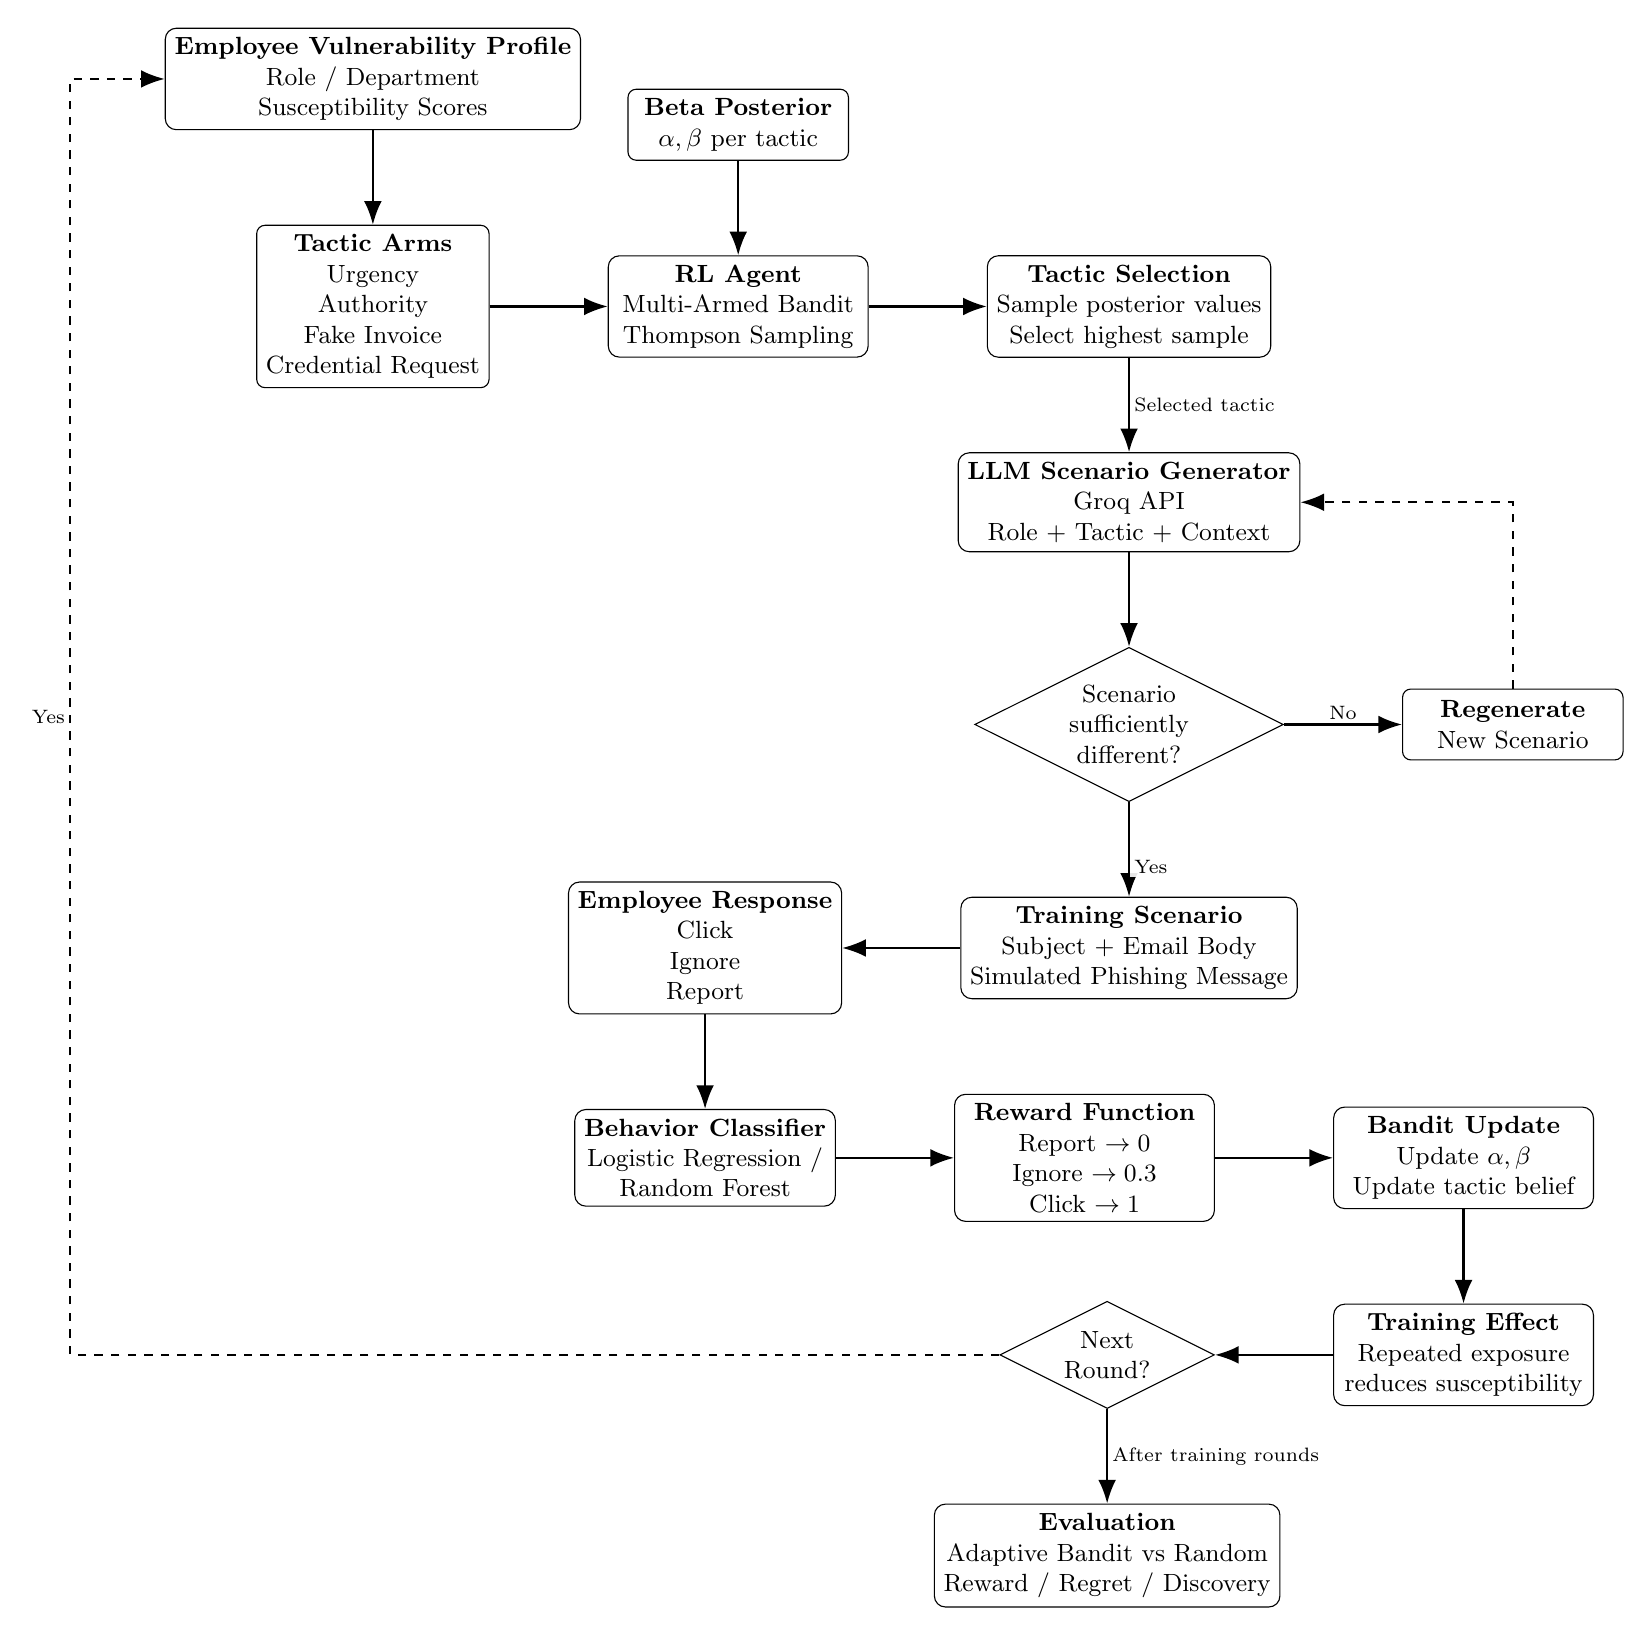
\begin{tikzpicture}[
    node distance=1.2cm and 1.5cm,
    box/.style={
        rectangle,
        rounded corners=4pt,
        draw,
        minimum width=3.3cm,
        minimum height=1.1cm,
        align=center,
        font=\small
    },
    smallbox/.style={
        rectangle,
        rounded corners=3pt,
        draw,
        minimum width=2.8cm,
        minimum height=0.9cm,
        align=center,
        font=\small
    },
    decision/.style={
        diamond,
        draw,
        aspect=2,
        align=center,
        font=\small,
        inner sep=2pt
    },
    arrow/.style={
        -{Latex[length=3mm]},
        thick
    },
    feedback/.style={
        -{Latex[length=3mm]},
        thick,
        dashed
    },
    flowlabel/.style={
        font=\scriptsize,
        fill=white,
        fill opacity=0.9,
        text opacity=1,
        inner sep=1.5pt
    }
]

\node[box] (profile) {
    \textbf{Employee Vulnerability Profile}\\
    Role / Department\\
    Susceptibility Scores
};

\node[smallbox, below=of profile] (tactics) {
    \textbf{Tactic Arms}\\
    Urgency\\
    Authority\\
    Fake Invoice\\
    Credential Request
};

\draw[arrow] (profile) -- (tactics);

\node[box, right=of tactics] (bandit) {
    \textbf{RL Agent}\\
    Multi-Armed Bandit\\
    Thompson Sampling
};

\draw[arrow] (tactics) -- (bandit);

\node[smallbox, above=of bandit] (posterior) {
    \textbf{Beta Posterior}\\
    $\alpha,\beta$ per tactic
};

\draw[arrow] (posterior) -- (bandit);

\node[box, right=of bandit] (selection) {
    \textbf{Tactic Selection}\\
    Sample posterior values\\
    Select highest sample
};

\draw[arrow] (bandit) -- (selection);

\node[box, below=of selection] (llm) {
    \textbf{LLM Scenario Generator}\\
    Groq API\\
    Role + Tactic + Context
};

\draw[arrow] (selection) --
    node[midway,right,flowlabel]{Selected tactic} (llm);

\node[decision, below=of llm] (fresh) {
    Scenario\\
    sufficiently\\
    different?
};

\draw[arrow] (llm) -- (fresh);

\node[smallbox, right=of fresh] (regenerate) {
    \textbf{Regenerate}\\
    New Scenario
};

\draw[arrow] (fresh) --
    node[midway,above,flowlabel]{No} (regenerate);
\draw[feedback] (regenerate.north) |- (llm.east);

\node[box, below=of fresh] (scenario) {
    \textbf{Training Scenario}\\
    Subject + Email Body\\
    Simulated Phishing Message
};

\draw[arrow] (fresh) --
    node[pos=0.68,right,flowlabel]{Yes} (scenario);

\node[box, left=of scenario] (employee) {
    \textbf{Employee Response}\\
    Click\\
    Ignore\\
    Report
};

\draw[arrow] (scenario) -- (employee);

\node[box, below=of employee] (classifier) {
    \textbf{Behavior Classifier}\\
    Logistic Regression /\\
    Random Forest
};

\draw[arrow] (employee) -- (classifier);

\node[box, right=of classifier] (reward) {
    \textbf{Reward Function}\\
    Report $\rightarrow 0$\\
    Ignore $\rightarrow 0.3$\\
    Click $\rightarrow 1$
};

\draw[arrow] (classifier) -- (reward);

\node[box, right=of reward] (update) {
    \textbf{Bandit Update}\\
    Update $\alpha,\beta$\\
    Update tactic belief
};

\draw[arrow] (reward) -- (update);

\node[box, below=of update] (training) {
    \textbf{Training Effect}\\
    Repeated exposure\\
    reduces susceptibility
};

\draw[arrow] (update) -- (training);

\node[decision, left=of training] (next) {
    Next\\
    Round?
};

\draw[arrow] (training) -- (next);

\coordinate (loopwest) at ([xshift=-1.2cm]profile.west);
\draw[feedback]
    (next.west) -- (loopwest |- next.west) --
    node[midway,left,flowlabel]{Yes}
    (loopwest) -- (profile.west);

\node[box, below=of next] (evaluation) {
    \textbf{Evaluation}\\
    Adaptive Bandit vs Random\\
    Reward / Regret / Discovery
};

\draw[arrow] (next) --
    node[midway,right,flowlabel]{After training rounds} (evaluation);

\end{tikzpicture}
}

\caption{Detailed design methodology of the proposed adaptive security awareness training system}
\label{fig:detailed_methodology}

\end{figure}

\clearpage
\begin{landscape}

\begin{figure}[H]
\centering
\includegraphics[
    width=0.98\linewidth,
    height=0.82\textheight,
    keepaspectratio
]{prism-uploads/adaptive_security_awareness_architecture2.drawio - Copy.png}
\caption{System architecture supporting the adaptive security awareness training methodology}
\label{fig:system_architecture}
\end{figure}

\end{landscape}
\clearpage


% =========================================================
% 7. ARCHITECTURE MODULES AND DESCRIPTION
% =========================================================

\section{Architecture Modules and Description}

The architecture is divided into a small set of modules, each with a
clear role in the training loop.

\subsection{Employee Vulnerability Profile}

The employee profile provides the context needed to personalize an
exercise. It stores the employee's synthetic role, department, response
history, and susceptibility to urgency, authority impersonation, fake
invoices, and credential requests. These values are hidden from the
bandit during evaluation so that it must learn from observed behavior.

\subsection{Reinforcement Learning Agent}

The reinforcement learning agent decides which tactic should be shown
next. Each tactic is represented as one bandit arm, and Thompson
Sampling maintains a probability distribution for every arm. Sampling
from these distributions gives less-tested tactics a chance to be
explored while still favouring tactics that have produced useful
feedback. After each round, the agent updates the distribution of the
selected tactic.

\subsection{LLM Scenario Generator}

The LLM scenario generator turns the selected tactic into a readable,
role-appropriate exercise rather than reusing the same fixed email. Its
input can include:

\begin{itemize}
    \item selected social-engineering tactic;
    \item employee role;
    \item department;
    \item scenario context; and
    \item previous scenario information.
\end{itemize}

Using this information, the module creates a fictional message for the
controlled training environment. The content is clearly treated as a
simulation and is never sent as a real phishing email.

\subsection{Behavior Classifier}

The behavior classifier provides a consistent way to interpret the
response produced by the employee simulator. A lightweight model such
as logistic regression or random forest can be trained on synthetic,
labeled examples, making the prototype practical to run on a standard
laptop.

Possible response classes include:

\begin{itemize}
    \item Click;
    \item Ignore;
    \item Report.
\end{itemize}

This classifier is only a component of the simulation. Its predictions
should not be presented as a validated model of real human behavior
without evidence from an appropriate human-participant study.

\subsection{Reward Function}

The reward function translates the classified response into a value the
learning agent can use. For vulnerability discovery, a risky response
produces a stronger internal signal:

\[
R(\text{report}) = 0
\]

\[
R(\text{ignore}) = 0.3
\]

\[
R(\text{click}) = 1
\]

This internal reward helps the agent locate tactics that deserve more
attention. It is separate from the learner-facing safety score, where
reporting a suspicious message is the preferred outcome. Keeping the
two measures distinct avoids rewarding unsafe behavior in the training
interface.

\subsection{Training Loop}

A complete round therefore follows these steps:

\begin{enumerate}
    \item Select a social-engineering tactic.
    \item Generate a contextualized scenario.
    \item Simulate the employee response.
    \item Classify the response.
    \item Calculate the reward.
    \item Update the bandit.
    \item Select the next tactic.
\end{enumerate}

\subsection{Dashboard and User Interface}

The implemented frontend provides separate workspaces for administrators
and employees. Administrators can view the organization risk overview,
manage training assignments, inspect model health, and review training
analytics. Employees can view their own assignments, personal progress,
training feedback, and active simulations.

The dashboard navigation was kept intentionally simple by removing the
unused Manage, Employees, Learning Path, Settings, and Preferences
sections. The remaining workspace links focus on the screens used by the
prototype. Risk graphs are shown in both workspaces with clearly labelled
axes: the horizontal axis represents training progress over time, while
the vertical axis represents the risk score from 0\% to 100\%. A lower
line indicates lower risk. The administrator view also includes a grey
comparison line representing performance without targeted training.


% =========================================================
% 8. DATASET DESCRIPTION
% =========================================================

\section{Dataset Description}

The prototype does not depend on an external public dataset. Instead,
it uses configurable synthetic employee profiles and records the
interactions generated during each experiment. Every simulated employee
is assigned a hidden susceptibility value for each social-engineering
tactic.

For example, a simplified profile may look like the following:

\begin{table}[H]
\centering
\caption{Example Simulated Employee Vulnerability Profile}
\label{tab:employeeprofile}

\begin{tabular}{lc}
\toprule
\textbf{Tactic} & \textbf{Susceptibility} \\
\midrule
Urgency & 0.30 \\
Authority impersonation & 0.45 \\
Fake invoice & 0.80 \\
Credential request & 0.25 \\
\bottomrule
\end{tabular}

\end{table}

Scenario-response examples for the behavior classifier are generated
from these profiles. A single training record can contain:

\begin{itemize}
    \item employee identifier;
    \item employee role;
    \item selected tactic;
    \item generated scenario;
    \item scenario features;
    \item simulated response;
    \item reward;
    \item training round.
\end{itemize}

Because the underlying susceptibility values are known, the synthetic
dataset makes it possible to check whether the bandit identifies the
intended weakness. At the same time, the results must be interpreted as
an algorithmic evaluation rather than evidence about real employees.


% =========================================================
% 9. RESULTS AND ANALYSIS
% =========================================================

\section{Results and Analysis}

The implemented prototype successfully connects the synthetic employee
profiles, Thompson Sampling policy, scenario generation, response
classification, and dashboard visualization into one training loop.
Each completed round records the selected tactic, scenario, response,
reward, and training progress. This allows the system to analyse both
individual performance and organization-level risk.

The administrator dashboard summarizes the number of employees, rounds
analysed, average reporting time, and repeat clickers. It also shows the
risk trend across training rounds and provides model-health information.
The employee dashboard presents assignments, personal risk progress,
feedback, and the next available simulation. In both dashboards, a
lower risk-score line represents safer performance over time.

The current results should be treated as prototype results rather than
general claims about human behaviour. The data is synthetic and is used
to verify that the software records interactions, updates the policy,
and presents the resulting trends correctly.


% =========================================================
% 10. EXPECTED OUTCOME
% =========================================================

\section{Expected Outcome}

The expected outcome is that the adaptive policy will identify tactics
that produce weaker responses and select them more often for targeted
practice. With repeated rounds, employees should receive more relevant
scenarios instead of following the same fixed sequence. The system is
also expected to generate varied, role-aware scenarios while keeping
the training process controlled and measurable.

Success will be assessed using the recorded reward, risk score,
reporting behaviour, tactic-selection frequency, and trend across
training rounds. The dashboard should make these changes understandable
to users without requiring them to interpret the internal bandit
parameters.


% =========================================================
% 11. COMPARISON ANALYSIS
% =========================================================

\section{Comparison Analysis}

The adaptive system is compared with a random tactic-selection
baseline. Both approaches use the same synthetic employee profiles,
number of training rounds, scenario-response process, and reward
calculation. The only difference is how the next tactic is selected.

\begin{table}[H]
\centering
\caption{Adaptive Policy and Random Baseline Comparison}
\label{tab:comparison}
\begin{tabularx}{\textwidth}{@{}lXX@{}}
\toprule
\textbf{Measure} & \textbf{Adaptive Thompson Sampling} & \textbf{Random selection} \\
\midrule
Tactic selection & Uses previous responses and rewards & Selects tactics without learning \\
Personalization & Gives more attention to observed weak areas & Gives similar exposure to all tactics \\
Exploration & Balances exploration and targeted practice & Has no policy-based balance \\
Scenario focus & Can concentrate on tactics needing more training & May repeat strong or weak tactics unpredictably \\
Expected learning value & More focused training over time & Useful as a simple reference point \\
\bottomrule
\end{tabularx}
\end{table}

The adaptive approach is expected to achieve a more informative reward
trend and faster discovery of the intended weakness than random
selection. The comparison does not prove that one method is better for
real employees; it only measures the behaviour of the two policies in
the controlled synthetic environment.


% =========================================================
% 12. CONCLUSION AND REFERENCES
% =========================================================

\section{Conclusion}

This project brings adaptive tactic selection, LLM-based scenario
generation, synthetic employee modeling, behavior classification, and
response-based feedback into one working training loop. Thompson
Sampling offers a transparent way to balance the exploration of less
tested tactics with the use of tactics that have already produced
useful evidence. The synthetic environment also provides a fair basis
for comparing this adaptive approach with random selection.

The implemented dashboard also provides separate administrator and
employee views with simplified navigation and clearer risk visualizations.
The graphs label the training timeline and risk-score axis so that users
can understand whether risk is increasing or decreasing without needing
to interpret technical model details.

The result is intended to be a practical proof of concept rather than
a validated model of employee psychology. It demonstrates how security
awareness training could respond to individual behavior while remaining
within a controlled, consent-based setting. No real phishing campaign
is conducted, and no real credentials are requested or collected.

\clearpage
\nocite{*}
\begingroup
\justifying
\setlength{\bibhang}{0.5in}
\setlength{\bibitemsep}{0.75\baselineskip}
\setlength{\emergencystretch}{2em}
\printbibliography[heading=bibintoc,title={References}]
\endgroup

\end{document}
